\documentclass[german]{latteachCD}
\usepackage{mdframed}
\usepackage{amsmath}
\usepackage{amsfonts}
\usepackage{amssymb}
%\usepackage{wasysym}
%\usepackage{stmaryrd}
%\usepackage{fixltx2e}
%\usepackage{enumitem}

\usepackage{tikz}
\usetikzlibrary{arrows}
\usetikzlibrary{automata}
\usetikzlibrary{positioning}
\usepackage{xspace}

\author{~}
\term{Wintersemester 2017/18}
\title{\Large 2.\@ Übungsblatt}
\course{\LARGE Formale Systeme}

\usepackage{csquotes}
\usepackage{booktabs}
\usepackage{amsmath}
\usepackage{amsfonts}
\usepackage{amssymb}
\usepackage{mathtools}
\usepackage{wasysym}
\usepackage{stmaryrd}
\usepackage{enumitem}
\usepackage{tikz}
\usepackage{makecmds}

\renewcommand{\epsilon}{\varepsilon}
\renewcommand{\phi}{\varphi}
\renewcommand{\rho}{\varrho}
\renewcommand{\theta}{\vartheta}
\newcommand{\tuple}[1]{\langle{#1}\rangle} 

\newcommand{\size}[1]{\ensuremath{\lvert #1\rvert}}
\newcommand{\gdw}{\mathrel{\mathrm{gdw.}}}
\newcommand{\falls}{\mathrel{\mathrm{falls}}}

\provideenvironment{solution}{\textbf{Lösung}:}{}
\usepackage{comment}

\usepackage{etex,etoolbox}

\DeclareRobustCommand{\NN}{\ensuremath{\mathbb{N}}}

\newbool{Baader}
\newbool{Kroetzsch}
\booltrue{Kroetzsch}

\DeclareMathOperator{\Var}{Var}
\ifbool{Baader}{%
  \DeclareMathOperator{\Unt}{Unt}
  \DeclareMathOperator{\Res}{Res}
}{}
\ifbool{Kroetzsch}{%
  \DeclareMathOperator{\Unt}{Sub}
  \DeclareMathOperator{\Res}{Res}
  \usepackage{multicol}         % for resolution
}{}

\excludecomment{solution}

\begin{document}

\maketitle

\begin{center}
\begin{mdframed}
  \renewcommand{\theexercise}{zur Selbstkontrolle
  (diese werden in den Übungen nicht besprochen)}
  
\begin{exercise}

\begin{enumerate}
\item[S3)] Wiederholen Sie die Begriffe:
  Alphabet, Wort, formale Sprache, Grammatik, Typ einer Grammatik, Typ einer Sprache,
  deterministischer endlicher Automat, nichtdeterministischer endlicher Automat und reguläre Sprache.
\item[S4)] Zeigen oder widerlegen Sie folgende Identität
\[
  ({L_1}^{*}\circ {L_2}^{*})^{*}=(L_1\cup L_2)^{*}\,.
\]
\end{enumerate}

\end{exercise}

%  {\bfseries Hinweis:} Die Aufgaben *) und **) 
%  dienen der Selbstkontrolle und werden in der
%  Übung nicht besprochen.  
\end{mdframed}
\end{center}

\setcounter{exercise}{0}


\begin{exercise}
Gegeben ist die Grammatik $G=(\{S,A,B,C,D\},\{a,b,c\},P,S)$ mit
\begin{eqnarray*}
  P & = & \{S\longrightarrow AB, S\longrightarrow C, S\longrightarrow \varepsilon, 
  A\longrightarrow aA,  A\longrightarrow \varepsilon, B\longrightarrow bBc,  B\longrightarrow Bc,  B\longrightarrow\varepsilon,\\
  & & C\longrightarrow aCc, C\longrightarrow Cc, C\longrightarrow D, D\longrightarrow aD, D\longrightarrow \varepsilon\}.
\end{eqnarray*}
Geben Sie eine zu $G$ äquivalente $\varepsilon$-freie Grammatik $G'$ an. 
\end{exercise}


\begin{exercise}
  Geben Sie jeweils einen DFA ${\mathcal{M}}_i$ an, der die Sprache $L_i$ akzeptiert: 
  \begin{enumerate}
   \item $L_1=\{a^nbac^m\mid \text{$m,n>0$, $n$ ist gerade und $m$ ist ungerade}\}$
   \item $L_2=\big\{w \in \{0,1\}^* \mid \exists i \in \{0,1\}, \text{ sodass } i \text{ Suffix von } w \text{ ist und } |w|_i \text{ mod } 2=1 \text{ gilt.}\big\}$
  \end{enumerate}
  Hierbei bezeichnet $|w|_i$ mit $i\in \{0,1\}$ die Anzahl an $i$'s in $w$.
\end{exercise}


\newpage

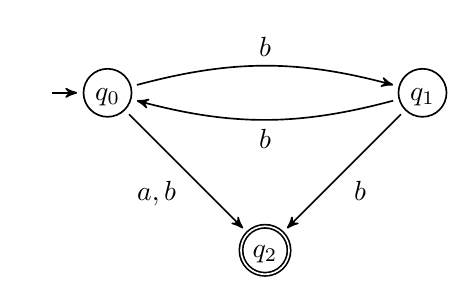
\begin{tikzpicture}[->,
        >=stealth',
        semithick,
        initial text=,
        shorten <=2pt,
        shorten >=2pt,
        auto,
        on grid,
        node distance=5ex and 5em,
        every state/.style={minimum size=0pt,inner sep=2pt,text height=1.5ex,text depth=.25ex},
        bend angle=15]

      \begin{scope}
        \node[state, initial]   (q_0) {$q_{0}$};
        \node[state]            (q_1) [right=4 of q_0] {$q_{1}$};
        \node[state, accepting] (q_2) [below right=2 and 2 of q_0] {$q_{2}$};

        \path
        (q_0) edge[bend left] node {$b$} (q_1)
        (q_1) edge[bend left] node {$b$} (q_0)
        (q_0) edge            node[below left] {$a,b$} (q_2)
        (q_1) edge            node {$b$} (q_2);
      \end{scope}

\end{tikzpicture}


\begin{exercise}
Beweisen oder widerlegen Sie unter Verwendung von Resultaten aus der Vorlesung folgende Aussagen.
\begin{enumerate}
\item Für jede reguläre Sprache $L$ kann eine kontextfreie 
  Grammatik $G$ mit $L=L(G)$ angegeben werden.
%\item Für jede kontextfreie Sprache $L$ kann eine reguläre 
%  Grammatik $G$ mit $L=L(G)$ angegeben werden.
\item Wenn $L$ von einem DFA erkannt werden kann und $L\subseteq L'$ gilt, 
  so kann $L'$ ebenfalls von einem DFA erkannt werden.
\item Wenn $L$  von einem DFA erkannt werden kann und $L'\subseteq L$ gilt, 
  so kann $L'$ ebenfalls von einem DFA erkannt werden.
\end{enumerate}
\end{exercise}


\begin{exercise}
  Gegeben ist der NFA
  $\mathcal{M}=(\{q_0,q_1,q_2,q_3,q_4,q_5\},\{a,b\},\delta ,\{q_0\}, \{q_3,q_4\})$ mit $\delta$:
  \begin{center}
  
\begin{exercise}
  Gegeben ist der NFA
  $\mathcal{M}=(\{q_0,q_1,q_2,q_3,q_4,q_5\},\{a,b\},\delta ,\{q_0\}, \{q_3,q_4\})$ mit $\delta$:
  \begin{center}
  
\begin{exercise}
  Gegeben ist der NFA
  $\mathcal{M}=(\{q_0,q_1,q_2,q_3,q_4,q_5\},\{a,b\},\delta ,\{q_0\}, \{q_3,q_4\})$ mit $\delta$:
  \begin{center}
  \input{pool/graphics/sprachen-nfa-grammatik}
  \end{center}
  Geben Sie eine reguläre Grammatik an, die die Sprache $L(\mathcal{M})$ erzeugt.
\end{exercise}

  \end{center}
  Geben Sie eine reguläre Grammatik an, die die Sprache $L(\mathcal{M})$ erzeugt.
\end{exercise}

  \end{center}
  Geben Sie eine reguläre Grammatik an, die die Sprache $L(\mathcal{M})$ erzeugt.
\end{exercise}


\end{document}
